\chapter{Formal Concept Analysis}
\label{chapter:formal-concept-analysis}

\FCA (henceforth initialised to FCA) is an approach to reasoning about \textit{concepts} and corresponding \textit{conceptual structures} in terms of lattice theory. At the foundation of FCA lies the philosophical
viewpoint, tracing back to Aristotle, which describes concepts as a unit consisting of two parts: the \textit{extension}, which refers to what one might refer to as instantiations of the concept, and the
\textit{intension}, which refers to the meaning we ascribe to a concept by virtue of its properties \cite{ganter1999formal, WILLE1992493, DUQUENNE1999407}.

\section{Basic Notions in Formal Concept Analysis}
\label{section:basic-notions}

The starting point in FCA is almost always a structure called a \textit{formal context}, or simply a \textit{context}. A context describes a universe of discourse, as well as the underlying structural
relationship that exists between elements in this universe.
%
\begin{definition}
  \index{formal context} \label{definition:formal-context} A formal context $\context = \GMI$ is a triple comprised of a set $G$ of objects , a set $M$ of attributes, and a binary relation
  $I \subseteq G \times M$ referred to as an `incidence' relation. For an object-attribute pair $(g,m) \in I$ we may say \say{The object $g$ \textit{has} the attribute $m$}.
\end{definition}

We regard the set of objects as being the extensional dimension of the context, while the set of attributes is intensional. However, this is largely convention; there is no strict requirement around what
these sets are made up of, or even that they be distinct. It is perfectly acceptable to have a context where the objects and attributes are the same set; for example, the context $(\mathbb{N}, \mathbb{N}
, \texttt{divides})$ which describes the division relationship between natural numbers. The choice of what constitutes an object or an attribute depends entirely on the desired interpretation and
purpose of the analysis. Thus, the distinction between extensional and intensional dimensions is largely for matters of intuition, rather than a strict requirement.

It should be noted that, while the presence of an object--attribute pair $(g,m)$ in the incidence relation is interpreted as the object satisfying the respective attribute, FCA is concerned only with
\textit{positive} information, and so the absence of a pair in the relation is not usually interpreted to mean that the object has the negation of the attribute. We will discuss, in more depth, the rather
troubling matter of negation and negative attributes in \Cref{section:contextual-attribute-logic}.

When the cardinalities of $G$ and $M$ are small, contexts may be represented as a cross-table such as in \Cref{cxt:grouplikes}. Each object is represented by a row in the table, each attribute by a
column, and each pair in the incidence relation is marked with an `$\times$' at the appropriate position \cite[pp. 17]{ganter1999formal}. Given a context that is presented in this form, it is quite a trivial
task to identify all the attributes that a particular object satisfies: one need only scan across the respective row and note where the marks appear. The resulting set of attributes is called the \textit{object's
intent}. The dual notion of an \textit{attribute extent} can be found by traversing down a column in the table.

\begin{figure}[H]
  \centering
  \small
  \begin{cxt}
    \label{cxt:grouplikes} \cxtName{\textbf{\texttt{Algebraic Structures}}} \att{\texttt{closure}} \att{\texttt{associativity}} \att{\texttt{identity}} \att{\texttt{divisibility}} \att{\texttt{commutativity}}
    \obj{x....}{\texttt{magma}} \obj{xx...}{\texttt{semigroup}} \obj{xxx..}{\texttt{monoid}} \obj{xxxx.}{\texttt{group}} \obj{xxxxx}{\texttt{abelian group}} \obj{x.xx.}{\texttt{loop}} \obj{x..x.}{\texttt{quasigroup}}
    \obj{.xxx.}{\texttt{groupoid}} \obj{.xx..}{\texttt{category}} \obj{.x...}{\texttt{semicategory}}
  \end{cxt}
  \caption{A formal context showing necessary properties of group-like structures.}
  \label{context:formal-context-group-structures}
\end{figure}

Using this approach, we can see that the intent of $\texttt{magma}$ is the singleton $\{\texttt{closure}\}$, while the extent of \texttt{closure} is the set
$\{\texttt{magma,semigroup,monoid,group,ableian group,loop,quasigroup}\}$.

This approach to determining object extents and attribute intents becomes impractical when considering non-trivial contexts, or large sets of objects and attributes. The procedure can be formally
described by the \textit{derivation operators}: \footnote{It is common to denote either derivation operator with a prime and use the surrounding context to resolve ambiguity, so $A^{\uparrow}$ and $B^{\downarrow}$
would become $A'$ and $B'$, respectively. We avoid this notation as later on it will become increasingly challenging to avoid ambiguity while maintaining pleasing notation. In cases where a derivation
operator is applied to a singleton of objects $\{g\}$ (\textit{resp.} attributes $\{m\}$) we omit the parenthesis and write $g^{\uparrow}$ (\textit{resp.} $m^{\downarrow}$)}

\begin{definition}
  \index{derivation operators} \label{definition:derivation-operators} Given a context $\GMI$, the \textit{derivation operators} are two maps $(\cdot)^{\uparrow}: \pset{G}\to \pset{M}$ and $(\cdot )^{\downarrow}
  : \pset{M}\to \pset{G}$. Then, for any subsets $A \subseteq G$ and $B \subseteq M$,
  \begin{align*}
    A^{\uparrow}   & \coloneqq \{m \in M \mid \forall g \in A, \; (g,m) \in I\} \\
    B^{\downarrow} & \coloneqq \{g \in G \mid \forall m \in B, \; (g,m) \in I\}
  \end{align*}
\end{definition}

The derivation operators describe a mapping from a subset $A \subseteq G$ of objects in a context to the corresponding subset of attributes that each (and every) object in $A$ related to. The dual notion
holds for starting with a subset of attributes. As an example, we might wish to determine the set of attributes satisfied by the objects $\{\texttt{group,groupoid,abelian group}\}$. Application of the
$(\cdot)^{\uparrow}$ derivation operator to this set yields $\{\texttt{associativity,identity,divisibility}\}$.

To offer another perspective on the derivation operators, obvserve that the derivation of a set $A\subseteq G$ of objects is the intersection of each object intent, and so we have
\begin{align*}
  A^{\uparrow}= \bigcap \{a^{\uparrow}\mid a \in A\}     & \qquad A \subseteq G  \\
  B^{\downarrow}= \bigcap \{b^{\downarrow}\mid b \in B\} & \qquad B \subseteq M.
\end{align*}

In fact, we have already explored a more general perspective on the derivation operators in \Cref{section:closure-systems} through the notion of closure operators and Galois connections. The proposition
below recontextualises properties of Galois connections in FCA.

\begin{proposition}
  \label{proposition:derivation-operators-galois} Let $\GMI$ be a formal context and consider the subsets $X,X_{1}\subseteq G$ of objects (\textit{resp.} $Y,Y_{1}\subseteq M$ of attributes) then
  \begin{align}
     & X \subseteq X_{1}\Rightarrow X_{1}^{\uparrow}\subseteq X^{\uparrow} & \textit{(resp.)}         & \qquad Y \subseteq Y_{1}\Rightarrow Y_{1}^{\downarrow}\subseteq Y^{\downarrow}\label{equation:galois-1} \\
     & X \subseteq X^{\uparrow \downarrow}                                 & \textit{(resp.)}         & \qquad Y \subseteq Y^{\downarrow \uparrow}\label{equation:galois-2}                                     \\
     & X^{\uparrow}= X^{\uparrow \downarrow \uparrow}                      & \textit{(resp.)}         & \qquad Y^{\downarrow}= Y^{\downarrow \uparrow \downarrow}\label{equation:galois-3}                      \\
     & X \subseteq Y^{\downarrow}\tiff X^{\uparrow}\supseteq Y             & \label{equation:galois-4}
  \end{align}
\end{proposition}

If we consider the powerset lattices of $\pset{G}$ and $\pset{M}$ under their usual inclusion orders, then the derivation operators constitute a Galois connection on these sets:
\Cref{equation:galois-1,equation:galois-2,equation:galois-3} are just a rephrasing of \Cref{equation:ord_galois-1,equation:ord-galois-2,equation:ord-galois-3}; while \Cref{equation:galois-4} rephrases
\Cref{proposition:fundamental-galois}. Mirroring the `discussion' on Galois connections, we obtain the closure systems $\mathcal{G}$ and $\mathcal{M}$ on $G$ and $M$, respectively. Each of these closure
systems form a complete lattice where, recounting \Cref{theorem:closure-systems-lattices}, meets and joins are given by:
%
\begin{align*}
   & \underset{i \in I}\bigwedge A_{i}= \underset{i \in I}\bigcap A_{i}\quad \text{ and }\quad \underset{i \in I}\bigvee A_{i}= \big(\underset{i \in I}\bigcup A_{i}\big)^{\uparrow \downarrow} & \quad A\subseteq \mathcal{G} \\
   & \underset{i \in I}\bigwedge B_{i}= \underset{i \in I}\bigcap B_{i}\quad \text{ and }\quad\underset{i \in I}\bigvee B_{i}= \big( \underset{i \in I}\bigcup B_{i}\big)^{\downarrow \uparrow} & \quad B\subseteq \mathcal{M}
\end{align*}

It follows \Cref{proposition:galois-connections-closure-operators} (and \Cref{figure:two-lattices} provides some visual intuition) that the closure systems induced by the derivation operators are dually
isomorphic to one another, and so each closed set of objects in $\mathcal{G}$ maps to a closed set of attributes in $\mathcal{M}$ and vice verse.
\vspace{-5em}
\begin{figure}[H]
  \centering
  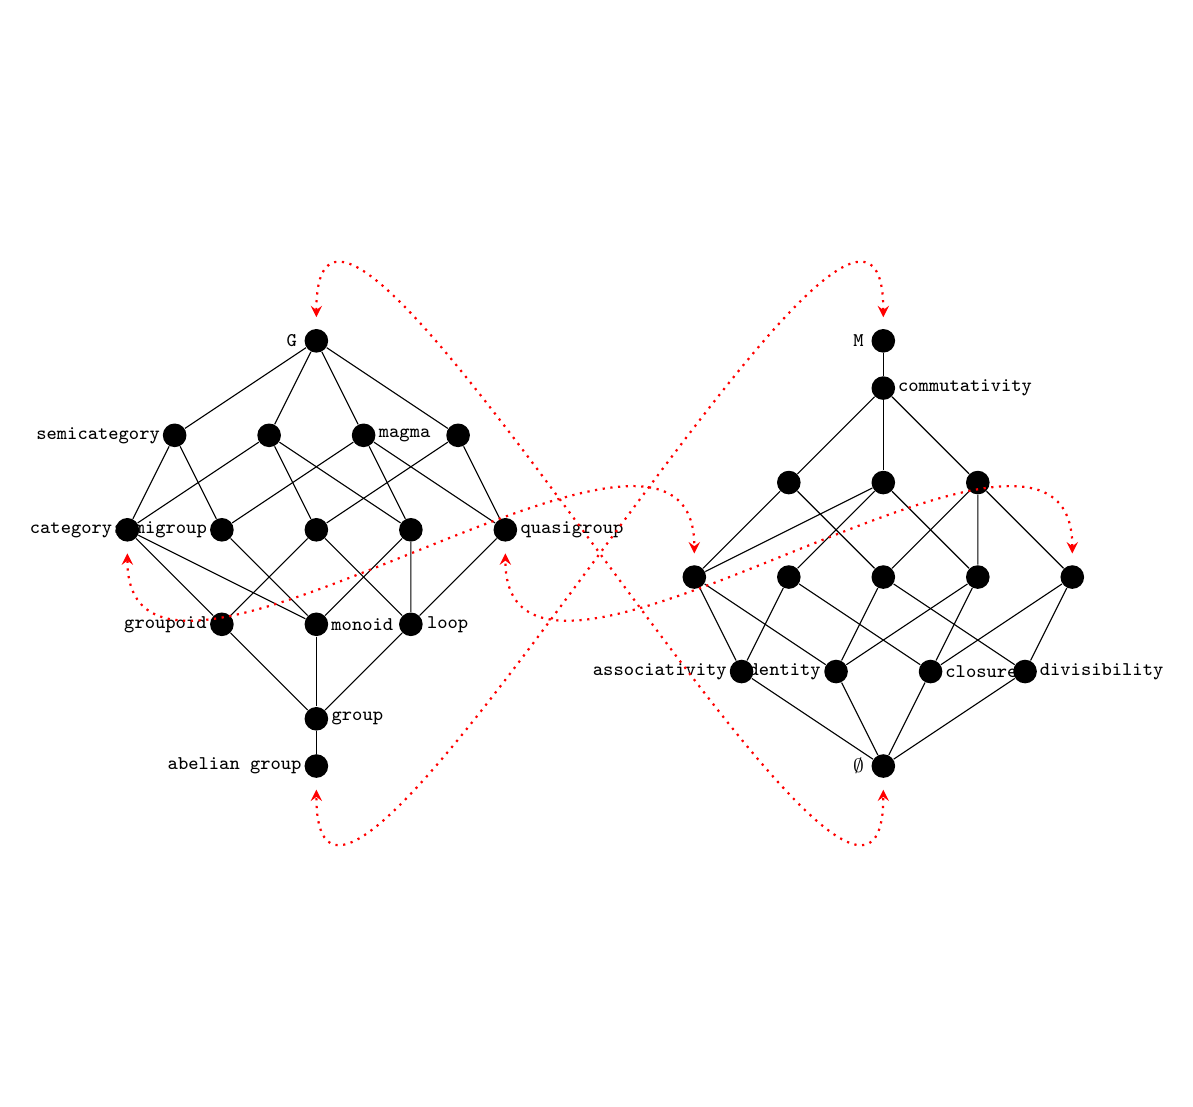
\begin{tikzpicture}[scale=0.6, every node/.style={circle, fill=black, inner sep=0.5pt, minimum size=3mm}]
    \node (a1) at (0,4) [label=left:{\scriptsize \texttt{G}}] {};

    \node (b1) at (-3,2) [label=left:{\scriptsize \texttt{semicategory}}] {};
    \draw (a1) -- (b1);

    \node (b2) at (-1,2) [label=left:{\scriptsize \texttt{}}] {};
    \draw (a1) -- (b2);

    \node (b3) at (1,2) [label=right:{\scriptsize \texttt{magma}}] {};
    \draw (a1) -- (b3);

    \node (b4) at (3,2) [label=right:{\scriptsize \texttt{}}] {};
    \draw (a1) -- (b4);

    \node (c1) at (-4,0) [label=left:{\scriptsize \texttt{category}}] {};
    \draw (c1) -- (b1);
    \draw (c1) -- (b2);

    \node (c2) at (-2,0) [label=left:{\scriptsize \texttt{semigroup}}] {};
    \draw (c2) -- (b1);
    \draw (c2) -- (b3);

    \node (c3) at (0,0) [label=left:{\scriptsize \texttt{}}] {};
    \draw (c3) -- (b2);
    \draw (c3) -- (b4);

    \node (c4) at (2,0) [label=right:{\scriptsize \texttt{}}] {};
    \draw (c4) -- (b2);
    \draw (c4) -- (b3);

    \node (c5) at (4,0) [label=right:{\scriptsize \texttt{quasigroup}}] {};
    \draw (c5) -- (b3);
    \draw (c5) -- (b4);

    \node (d1) at (-2,-2) [label=left:{\scriptsize \texttt{groupoid}}] {};
    \draw (d1) -- (c1);
    \draw (d1) -- (c3);

    \node (d2) at (0,-2) [label=right:{\scriptsize \texttt{monoid}}] {};
    \draw (d2) -- (c1);
    \draw (d2) -- (c2);
    \draw (d2) -- (c4);

    \node (d3) at (2,-2) [label=right:{\scriptsize \texttt{loop}}] {};
    \draw (d3) -- (c3);
    \draw (d3) -- (c4);
    \draw (d3) -- (c5);

    \node (e1) at (0,-4) [label=right:{\scriptsize \texttt{group}}] {};
    \draw (e1) -- (d1);
    \draw (e1) -- (d2);
    \draw (e1) -- (d3);

    \node (f1) at (0,-5) [label=left:{\scriptsize \texttt{abelian group}}] {};
    \draw (f1) -- (e1);

    \begin{scope}[shift={(12,0)}]
      \node (ra1) at (0,-5) [label=left:{\scriptsize $\emptyset$}] {};

      \node (rb1) at (-3,-3) [label=left:{\scriptsize \texttt{associativity}}] {};
      \draw (ra1) -- (rb1);

      \node (rb2) at (-1,-3) [label=left:{\scriptsize \texttt{identity}}] {};
      \draw (ra1) -- (rb2);

      \node (rb3) at (1,-3) [label=right:{\scriptsize \texttt{closure}}] {};
      \draw (ra1) -- (rb3);

      \node (rb4) at (3,-3) [label=right:{\scriptsize \texttt{divisibility}}] {};
      \draw (ra1) -- (rb4);

      \node (rc1) at (-4,-1) [label=left:{\scriptsize \texttt{}}] {};
      \draw (rc1) -- (rb1);
      \draw (rc1) -- (rb2);

      \node (rc2) at (-2,-1) [label=left:{\scriptsize \texttt{}}] {};
      \draw (rc2) -- (rb1);
      \draw (rc2) -- (rb3);

      \node (rc3) at (0,-1) [label=left:{\scriptsize \texttt{}}] {};
      \draw (rc3) -- (rb2);
      \draw (rc3) -- (rb4);

      \node (rc4) at (2,-1) [label=right:{\scriptsize \texttt{}}] {};
      \draw (rc4) -- (rb2);
      \draw (rc4) -- (rb3);

      \node (rc5) at (4,-1) [label=right:{\scriptsize \texttt{}}] {};
      \draw (rc5) -- (rb3);
      \draw (rc5) -- (rb4);

      \node (rd1) at (-2,1) [label=left:{\scriptsize \texttt{}}] {};
      \draw (rd1) -- (rc1);
      \draw (rd1) -- (rc3);

      \node (rd2) at (0,1) [label=right:{\scriptsize \texttt{}}] {};
      \draw (rd2) -- (rc1);
      \draw (rd2) -- (rc2);
      \draw (rd2) -- (rc4);

      \node (rd3) at (2,1) [label=right:{\scriptsize \texttt{}}] {};
      \draw (rd3) -- (rc3);
      \draw (rd3) -- (rc4);
      \draw (rd3) -- (rc5);

      \node (re1) at (0,3) [label=right:{\scriptsize \texttt{commutativity}}] {};
      \draw (re1) -- (rd1);
      \draw (re1) -- (rd2);
      \draw (re1) -- (rd3);

      \node (rf1) at (0,4) [label=left:{\scriptsize \texttt{M}}] {};
      \draw (rf1) -- (re1);
    \end{scope}
    \draw[red, dotted, stealth-stealth, line width=0.8pt] (12,4.5) to[out=90, in=270] (0,-5.5);
    \draw[red, dotted, stealth-stealth, line width=0.8pt] (16,-0.5) to[out=90, in=270] (4,-0.5);
    \draw[red, dotted, stealth-stealth, line width=0.8pt] (-4,-0.5) to[out=270, in=90] (8,-0.5);
    \draw[red, dotted, stealth-stealth, line width=0.8pt] (0,4.5) to[out=90, in=270] (12,-5.5);
  \end{tikzpicture}
  \vspace{-6em}
  \caption{The lattices for the closure systems $\mathcal{G}$ and $\mathcal{M}$, respectively. We partially demonstrate the dual isomorphism between these structures. We read set inclusion from below.}
  \label{figure:two-lattices}
\end{figure}

Earlier, it was claimed that Galois connections are particularly interesting when the closure systems they induce are themselves interesting; and, future discussion of an example of such interesting closure
systems was promised. Let us now give such an example, and in doing so provide some intution for why Galois connections are a useful way of modelling concepts, to be introduced immediately afterwards!

Consider the concept derived from the algebraic structure of a `monoid': a set equipped with a binary operation that satisfies the properties of closure, associativity, and that has an identity element.
It would be ideal to include in the extension of this concept all those algebraic structures that fall under the subclass of monoids; that is, nothing more and nothing less than those structures that
satisfy closure, associativity, and have an identity element. It is completely obvious to point out that monoids should be included in this extension. Another structure which would be included in this
concept's extension is that of a `group': a set equipped with a binary operation satisfying all the properties of a monoid alongside the additional property of divisibility.

Now let us consider the concept derived from a `group'; we have just shown that a group is a subclass of monoid, so it should follow that the extension of a group must be a subset of the extension of a
monoid, but what of the intension? Suppose the intension of the concept of a monoid were not a subset of that of a group, then monoids would have to satisfy some property that groups did not. This is a
problem, as it suggests we should not have considered a group to be a subclass of a monoid.

It is finally an appropriate time to define what is meant by \textit{formal concept}:

\begin{definition}
  \index{formal concept} \index{lattice! concept lattice} \label{definition:formal-concept} A \emph{formal concept} of a context $\GMI$ is a pair $(A,B)$ where $A \subseteq G$ and $B\subseteq M$ where
  $A^{\uparrow}= B$ and $B^{\downarrow}= A$. We call $A$ the \emph{concept extent} and $B$ the \emph{concept intent}. We write $\BGMI$ to denote the set of all concepts of $\GMI$.
\end{definition}

Concepts are thus pairs of closed sets, where each set represents either the extensional or intensional perspective on the concept. In case it is not clear from the definition of formal concepts why
the concept extents and concept intents are necessarily closed, consider the following remark:

\begin{remark}
  We have established that the two closure operators $(\cdot)^{\uparrow \downarrow}$ and $(\cdot)^{\downarrow \uparrow}$ form a Galois connection, inducing the closure systems $\mathcal{G}$ and
  $\mathcal{M}$, respectively. It is (perhaps) not immediately obvious that, in fact, the image of the single operator $(\cdot)^{\uparrow}\colon \pset{G}\to \pset{M}$ coincides precisely with the set
  $\mathcal{M}$, and the image of $(\cdot)^{\downarrow}\colon \pset{M}\to \pset{G}$ similarly coincides with $\mathcal{G}$. This is a direct result of \Cref{equation:galois-3}, since any element in the
  derivation operators co-domain will be a closed set.
\end{remark}

One pleasing result stemming from this point is that, for any set $A\subseteq G$ of objects, the set $A^{\uparrow}$ will always be a concept intent, and may furthermore lead to the construction of $(A^{\uparrow
\downarrow}, A^{\uparrow})$ which is always a concept. The same idea holds so that for a set $B \subseteq M$ of attributes, $B^{\downarrow}$ is always a concept extent. We are even more fortunate in
that we have already described and discussed the structure of the collection of all concept intents (or extents)! These are merely the closure systems $\mathcal{G}$ and $\mathcal{M}$.

To clarify the earlier example of the concept of a `monoid', consider that the derivation $\{\texttt{monoid}\}^{\uparrow}$ yields the set of attributes $\{\texttt{closure,associativity,identity}\}$. In
turn, the derivation of this attribute set yields the set of objects $\{\texttt{monoid,group,abelian group}\}$. We know by properties of the Galois connection (specifically, \Cref{equation:galois-3})
that these two derived sets are closed with respect to the closure systems $\mathcal{M}$ and $\mathcal{G}$, and so
\[
  \big(\{\texttt{monoid,group,abelian group}\}, \{\texttt{closure,associativity,identity}\}\big)
\]
is a formal concept of \Cref{cxt:grouplikes}.

\begin{figure}[H]
  \centering
  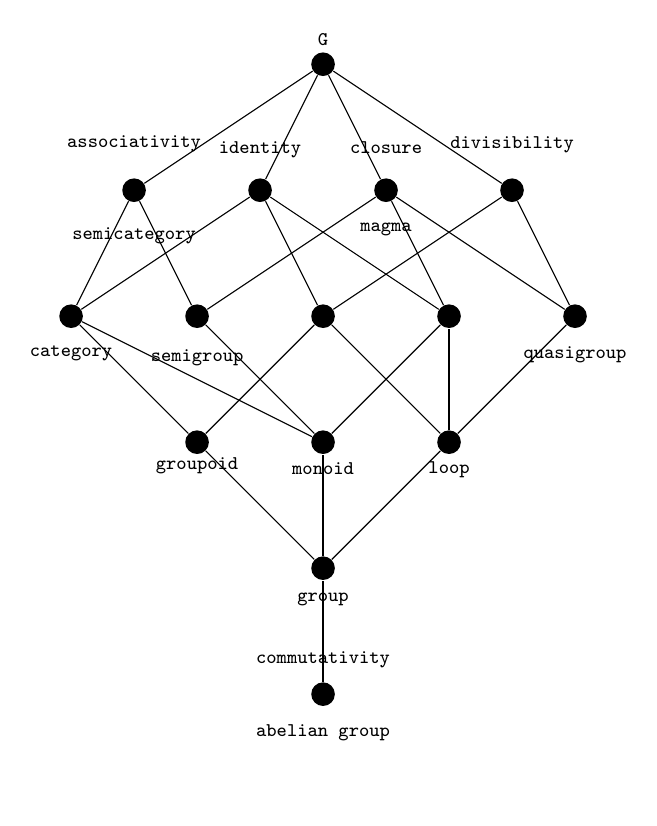
\begin{tikzpicture}[scale=0.8, every node/.style={circle,fill=black,inner sep=0.5pt,minimum size=3mm}]
    %––––– row 1 –––––
    \node (a1) at (0,4) [label={[anchor=south,yshift=0mm]above:{\scriptsize\texttt{G}}}] {};

    %––––– row 2 –––––
    \node (b1)
      at
      (-3,2)
      [label={[anchor=south,yshift=-4.5mm]above:{\scriptsize\texttt{associativity}}}, label={[anchor=north,yshift=4.5mm,text depth=0pt]below:{\scriptsize\strut\texttt{semicategory}}}]
      {};
    \draw (a1) -- (b1);

    \node (b2) at (-1,2) [label={[anchor=south,yshift=-2mm]above:{\scriptsize\texttt{identity}}}] {};
    \draw (a1) -- (b2);

    \node (b3) at (1,2) [label={[anchor=south,yshift=-1mm]above:{\scriptsize\texttt{closure}}}, label={[anchor=north,yshift=1mm,text depth=0pt]below:{\scriptsize\strut\texttt{magma}}}] {};
    \draw (a1) -- (b3);

    \node (b4) at (3,2) [label={[anchor=south,yshift=-4mm]above:{\scriptsize\texttt{divisibility}}}] {};
    \draw (a1) -- (b4);

    %––––– row 3 –––––
    \node (c1) at (-4,0) [label={[anchor=north,yshift=3mm,text depth=0pt]below:{\scriptsize\strut\texttt{category}}}] {};
    \draw (c1) -- (b1);
    \draw (c1) -- (b2);

    \node (c2) at (-2,0) [label={[anchor=north,yshift=3mm,text depth=0pt]below:{\scriptsize\strut\texttt{semigroup}}}] {};
    \draw (c2) -- (b1);
    \draw (c2) -- (b3);

    \node (c3) at (0,0) {};
    \draw (c3) -- (b2);
    \draw (c3) -- (b4);

    \node (c4) at (2,0) {};
    \draw (c4) -- (b2);
    \draw (c4) -- (b3);

    \node (c5) at (4,0) [label={[anchor=north,yshift=4mm,text depth=0pt]below:{\scriptsize\strut\texttt{quasigroup}}}] {};
    \draw (c5) -- (b3);
    \draw (c5) -- (b4);

    %––––– row 4 –––––
    \node (d1) at (-2,-2) [label={[anchor=south,yshift=-7mm]below:{\scriptsize\texttt{groupoid}}}] {};
    \draw (d1) -- (c1);
    \draw (d1) -- (c3);

    \node (d2) at (0,-2) [label={[anchor=south,yshift=-6mm]below:{\scriptsize\texttt{monoid}}}] {};
    \draw (d2) -- (c1);
    \draw (d2) -- (c2);
    \draw (d2) -- (c4);

    \node (d3) at (2,-2) [label={[anchor=south,yshift=-5mm]below:{\scriptsize\texttt{loop}}}] {};
    \draw (d3) -- (c3);
    \draw (d3) -- (c4);
    \draw (d3) -- (c5);

    %––––– row 5 –––––
    \node (e1) at (0,-4) [label={[anchor=south,yshift=-6mm]below:{\scriptsize\texttt{group}}}] {};
    \draw (e1) -- (d1);
    \draw (e1) -- (d2);
    \draw (e1) -- (d3);

    %––––– row 6 –––––
    \node (f1)
      at
      (0,-6)
      [label={[anchor=south,yshift=-6mm]above:{\scriptsize\texttt{commutativity}}}, label={[anchor=north,yshift=6mm,text depth=0pt]below:{\scriptsize\strut\texttt{abelian group}}}]
      {};
    \draw (f1) -- (e1);
  \end{tikzpicture}
  \caption{The concept lattice corresponding to \Cref{cxt:grouplikes}}
  \label{figure:concept-lattice-group-likes}
\end{figure}

\begin{remark}
  Reading a concept lattice requires a small amount of getting used to: the labels above a node in the diagram correspond to attributes, while objects are labelled below a node. Each node represents a
  concept $C \in \BGMI$. The extension of $C$ contains all objects attached to nodes which have a (strictly) downwards path from $C$, while the intension of $C$ contains those attributes labelled at
  nodes where there is a strictly upwards path from $C$.
\end{remark}

The set of concepts has a naturally arising partial order described by the \textit{subconcept--superconcept} relation. If $(A_{0},B_{0})$ and $(A_{1},B_{1})$ are two concepts in $\BGMI$, then
$(A_{0},B_{0})$ is a \textit{subconcept} of $(A_{1}, B_{1})$ and $(A_{1}, B_{1})$ is a superconcept of $(A_{0},B_{0})$ if and only if $A_{0}\subseteq A_{1}$; or, equivalently if $B_{1}\subseteq B_{0}$.
We write $\CLGMI$ to denote the set of concepts equipped with this partial ordering, and call this set the \textit{concept lattice}.

\begin{theorem}[The Basic Theorem of Concept Lattices]
  \label{theorem:basic-theorem} The concept lattice $\CLGMI$ of a formal context is a complete lattice in which meets and joins are given by
  \begin{align*}
     & \underset{i \in I}\bigwedge (A_{i}, B_{i}) = \Big( \underset{i \in I}\bigcap A_{i}, (\underset{i \in I}\bigcup B_{i})^{\downarrow \uparrow}\Big) \\
     & \underset{i \in I}\bigvee (A_{i}, B_{i}) = \Big( (\underset{i \in I}\bigcap A_{i})^{\uparrow \downarrow}), \underset{i \in I}\bigcup B_{i}\Big)
  \end{align*}
\end{theorem}

\section{Contextual Attribute Logic}
\label{section:contextual-attribute-logic}

The attribute logic that usually underlies any discussion on FCA is analogous to Horn logic. Attribute implications are quite easily shown to be analogous to propositional Horn clauses: If we consider
the (attribute) implication $A \rightarrow B$, with $A, B \subseteq M$ it can be phrased, with respect to holding in a context $\GMI$, as \say{all objects which satisfy every attribute in $A$ also satisfy every attribute in $B$}.

The underlying logic we have just described for FCA can quite easily be shown to be analogous to propositional Horn logic. Horn rules are syntactically similar to material implications, and share the
same `$\rightarrow$' operator. However, none of the premise nor conclusion of a Horn rule may be negative, or contain disjunction. They are not able to express what is \textit{not} a consequence of a premise.

waerawer the (attribute) implication $A \rightarrow B$, with $A, B \subseteq M$ it can be phrased, with respect to holding in a context $\GMI$, as \say{all objects which satisfy every attribute in $A$ also satisfy every attribute in $B$}.
waerawer the (attribute) implication $A \rightarrow B$, with $A, B \subseteq M$ it can be phrased, with respect to holding in a context $\GMI$, as \say{all objects which satisfy every attribute in $A$ also satisfy every attribute in $B$}.

% \begin{lemma}
%   \label{lemma:surjective-operators} Let $\GMI$ be a context with $(\uparrow, \downarrow)$ as the usual derivation operators. The closure systems
%   \[
%     \mathcal{G}\;=\; \{\,A\subseteq G \mid A^{\uparrow\downarrow}=A\,\}, \qquad \mathcal{M}\;=\; \{\,B\subseteq M \mid B^{\downarrow\uparrow}=B\,\}
%   \]
%   Then
%   \[
%     \mathcal{M}\;=\; \{\,A^{\uparrow}\mid A\subseteq G\,\}, \qquad \mathcal{G}\;=\; \{\,B^{\downarrow}\mid B\subseteq M\,\},
%   \]
%   and so $(\cdot)^{\uparrow}$ and $(\cdot)^{\downarrow}$ are surjective onto $\mathcal{M}$ and $\mathcal{G}$, respectively.
% \end{lemma}

% \begin{proof}
%   \label{proof:surjective-operators} We prove the statement for $(\cdot)^{\uparrow}$; the dual argument follows by swapping $G$ with $M$ and $\uparrow$ with $\downarrow$. Let $B \in \mathcal{M}$, then
%   by definition $B = B^{\downarrow \uparrow}$. Let some $A \subseteq G$ so that $A = B^{\downarrow}$.
% \end{proof}

% % To make formal the earlier example, $\big(\{\texttt{monoid,group,abelian group}\}, \{\texttt{closure,associativity,identity}\} \big)$ is a concept of the context in \Cref{cxt:grouplikes}.
% \textcolor{red}{I want to say something about how each operator is a map onto the closure system for its codomain. The next paragraph follows from this remark}

% From the Galois connection, for every subset $A\subseteq G$ of objects, the derivation $A^{\uparrow}$ of the subset is precisely a concept intent, and so $(A^{\uparrow \downarrow}, A^{\uparrow})$ always
% describes a concept. If this is not immediately obvious, consider that the derivation operator $(\cdot)^{\uparrow}\colon \pset{G}\to \pset{M}$ is onto the closure system $\mathcal{M}$, and can be
% described by
% %
% \begin{align*}
%   A^{\uparrow}= \bigcap \; \{g^{\uparrow}\mid g \in A \}
% \end{align*}

% Each object $g \in A$ is mapped to its object intent $g^{\uparrow}$ for which $g^{\uparrow}\in \mathcal{M}$, since $\mathcal{M}$ is closed under arbitrary intersections it follows that
% $A^{\uparrow}\in \mathcal{M}$, and so $A^{\uparrow}$ is closed.

% \clearpage
% Since $(\uparrow, \downarrow)$ constitute a Galois connection on the powersets $\pset{G}$ and $\pset{M}$, we can find two closure systems on $G$ and $M$, respectively.

% From \Cref{proposition:derivation-operators-galois} we can describe two closure operators $(\cdot)^{\uparrow \downarrow}$ and $(\cdot)^{\downarrow \uparrow}$ on the powersets $\pset{G}$ and $\pset{M}$,
% respectively.

% And so, $A^{\uparrow \downarrow}$---which can rather cumbersomely be described as \say{The set of all objects which satisfy all the attributes satisfied by \texttt{semigroup} and \texttt{monoid}}---would
% yield the set $\{\texttt{semigroup, monoid, group, abelian group}\}$. In fact, this composition of derivation operators satisfies very specific properties.%

% With the above relationship between sets of objects and attributes in mind, it is appropriate to introduce a \textit{formal concept}.

% It is no coincidence, as we will see later on, that this corresponds to taking the intersection of each object's intent, and so we have equivalently for a set of objects $A \subseteq G$

% \begin{align*}
%   A^{\uparrow}= \bigcap \{g^{\uparrow}\mid g \in A \} \quad \textit{(resp.)}\quad B^{\downarrow}= \bigcap \{m^{\downarrow}\mid m \in B\}
% \end{align*}

% \begin{example}
%   \label{example:formal-concept} If we consider the \texttt{groupoid} object from \Cref{cxt:grouplikes}, we can derive the concept:

%   \[
%     \big(\{\texttt{groupoid,group,abelian group}\}, \{\texttt{associativity,identity,closure }\} \big)
%   \]

%   % The derivation of \texttt{groupoid} yields $\{\texttt{associativity,identity,closure}\}$, by \Cref{equation:galois-3} this set is closed under its Galois connection, and formsc a concept intent.

%   % To begin, the object intent $\texttt{groupoid}^\uparrow$ is determined, which yields the set $\{\texttt{associativity,identity,closure}\}$. From \Cref{proposition:properties-about-derivation-operators} this set is closed, and represents a concept intent. The concept extent is determined by application of a derivation operator to the concept intent.
% \end{example}

% The set of all concepts has a natural ordering induced on it by the \textit{subconcept--superconcept} relation. If $(A_{0},B_{0})$ and $(A_{1},B_{1})$ are two concepts, then $(A_{0},B_{0})$ is a
% \textit{subconcept} of $(A_{1}, B_{1})$ and $(A_{1}, B_{1})$ is a superconcept of $(A_{0},B_{0})$ if and only if $A_{0}\subseteq A_{1}$. Equivalently if $B_{1}\subseteq B_{0}$. We denote set of all concepts
% ordered in this way by $\CLGMI$, and call this set the \textit{concept lattice} of $\GMI$.

% Intuitively, one concept is a subconcept of another, if every instance of the first concept is also an instance of the second. From the Galois connection, this is equivalently, albeit less intuitively,
% explained by every attribute of the second concept being included in the first.

% We can prescribe a rather intuitive ordering over concepts induced by the \textit{subconcept–superconcept} relation.
% \begin{figure}[H]
%   \centering
%   \begin{tikzpicture}[scale=0.8, every node/.style={circle, fill=black, inner sep=0.5pt,minimum size=0mm}]
%     \node (a1) at (0,3) [label=above:{\scriptsize $\top$}] {w};
%     % \node[draw=none, fill=none] at (0,3.5) {\tiny Top};

%     \node (b1) at (-3,1) [label=above:{\scriptsize \texttt{associativity}}] {};
%     \draw (a1) -- (b1);

%     \node (b2) at (-1,1) [label=above:{\scriptsize \texttt{identity}}] {z};
%     \draw (a1) -- (b2);

%     \node (b3) at (1,1) [label=above:{\scriptsize \texttt{closure}}, label=below:{\scriptsize \texttt{magma}}] {};
%     \draw (a1) -- (b3);

%     \node (b4) at (3,1) [label=above:{\scriptsize \texttt{divisibility}}] {};
%     \draw (a1) -- (b4);

%     \node (c1) at (-4,-1) [label=below:{\scriptsize \texttt{category}}] {};
%     \draw (c1) -- (b1);
%     \draw (c1) -- (b2);

%     \node (c2) at (-2,-1) [label=below:{\scriptsize \texttt{semigroup}}] {};
%     \draw (c2) -- (b1);
%     \draw (c2) -- (b3);

%     \node (c3) at (0,-1) {};
%     \draw (c3) -- (b2);
%     \draw (c3) -- (b3);

%     \node (c4) at (2,-1) {};
%     \draw (c4) -- (b2);
%     \draw (c4) -- (b4);

%     \node (c5) at (4,-1) [label=below:{\scriptsize \texttt{quasigroup}}] {};
%     \draw (c5) -- (b3);
%     \draw (c5) -- (b4);

%     \node (d1) at (-2,-3) [label=below:{\scriptsize \texttt{monoid}}] {};
%     \draw (d1) -- (c1);
%     \draw (d1) -- (c2);
%     \draw (d1) -- (c3);

%     \node (d2) at (0,-3) [label=below:{\scriptsize \texttt{groupoid}}] {};
%     \draw (d2) -- (c1);
%     \draw (d2) -- (c3);

%     \node (d3) at (2,-3) [label=below:{\scriptsize \texttt{loop}}] {};
%     \draw (d3) -- (c3);
%     \draw (d3) -- (c4);
%     \draw (d3) -- (c5);

%     \node (e1) at (0,-5) [label=below:{\scriptsize \texttt{group}}] {};
%     \draw (e1) -- (d1);
%     \draw (e1) -- (d2);
%     \draw (e1) -- (d3);

%     \node (f1) at (0,-7) [label=above:{\scriptsize \texttt{commutativity}}, label=below:{\scriptsize \texttt{abelian group}}] {};
%     \draw (f1) -- (e1);
%   \end{tikzpicture}
%   \caption{The concept lattice associated with the formal context in \Cref{cxt:grouplikes}}
% \end{figure}

% \subsection{Attribute Implications}
% \label{subsection:attribute-implications}

% In FCA, attribute implications represent dependencies that exist between attributes in a context. If $M$ is a non-empty set of attributes with $A, B \subseteq M$, then we denote an attribute
% implication over $M$ as $A \rightarrow B$.

% \begin{definition}
%   \label{definition:attribute-implication} Let $M$ be a non-empty set of attributes, then an \emph{attribute implication} over $M$ is a
% \end{definition}

% If we examine the context in \Cref{context:voting-records-small} it is apparent that every representative who voted in favour of the proposed crime bill also voted in favour of the immigration bill;
% we write this dependency as $\texttt{crime }\rightarrow \texttt{immigration}$.

% \begin{figure}[H]
%   \centering
%   \begin{cxt}
%     \cxtName{\textbf{\texttt{Congressional Voting Records}}} \atr{\texttt{mx-missile}} \atr{\texttt{crime}} \atr{\texttt{immigration}} \atr{\texttt{satellite ban}} \atr{\texttt{education}} \atr{\texttt{republican}}
%     \atr{\texttt{democrat}} \obj{.xx.xx.}{\texttt{Representative 1}} \obj{......x}{\texttt{Representative 4}} \obj{.x..xx.}{\texttt{Representative 9}} \obj{..x.x.x}{\texttt{Representative 17}}
%   \end{cxt}
%   \caption{A context describing a portion of congressional voting records for 1984}
%   \label{context:voting-records-small}
% \end{figure}

% \clearpage

% \begin{figure}[H]
%   \centering
%   \small
%   \begin{cxt}
%     \label{cxt:people} \cxtName{\textbf{\texttt{Characters}}} \att{\texttt{human}} \att{\texttt{tralfamadorian}} \att{\texttt{linear time}} \att{\texttt{soldier}} \att{\texttt{optometrist}} \att{\texttt{pacifist}}
%     \obj{x..xxx}{\texttt{Billy Pilgrim}} \obj{x.xx..}{\texttt{Edgar Derby}} \obj{x....x}{\texttt{Montana Wildhack}} \obj{.x....}{\texttt{Zookeeper}}\obj{x.xx..}{\texttt{Paul Lazzaro}} \obj{x.x.x.}{\texttt{Lionel Merble}}
%     \obj{.x.x..}{\texttt{Test Pilot}}
%   \end{cxt}
%   \caption{A formal context showing necessary properties of group-like structures.}
% \end{figure}

% \begin{figure}[H]
%   \centering
%   \begin{tikzpicture}[scale=0.6, every node/.style={circle, fill=black, inner sep=0.5pt, minimum size=0mm}]
%     \node (a1) at (0,4) [label=left:{\scriptsize \texttt{G}}] {w};

%     \node (b1) at (-2,2) [label=left:{\scriptsize \texttt{}}] {};
%     \draw (a1) -- (b1);

%     \node (b2) at (0,2) [label=left:{\scriptsize \texttt{}}] {z};
%     \draw (a1) -- (b2);

%     \node (b3) at (2,2) [label=right:{\scriptsize \texttt{zookeeper}}] {};
%     \draw (a1) -- (b3);

%     \node (c1) at (-4,0) [label=left:{\scriptsize \texttt{montanna}}] {};
%     \draw (c1) -- (b1);

%     \node (c2) at (-2,0) [label=left:{\scriptsize \texttt{}}] {};
%     \draw (c2) -- (b1);
%     \draw (c2) -- (b2);

%     \node (c3) at (-0,0) [label=left:{\scriptsize \texttt{}}] {};
%     \draw (c3) -- (b1);

%     \node (c4) at (2,0) [label=right:{\scriptsize \texttt{}}] {};
%     \draw (c4) -- (b1);

%     \node (c5) at (4,0) [label=right:{\scriptsize \texttt{quasigroup}}] {};
%     \draw (c5) -- (b2);
%     \draw (c5) -- (b3);

%     \node (d1) at (-2,-2) [label=left:{\scriptsize \texttt{edgar,paul}}] {};
%     \draw (d1) -- (c2);
%     \draw (d1) -- (c4);

%     \node (d2) at (1,-2) [label=right:{\scriptsize \texttt{lionel}}] {};
%     \draw (d2) -- (c3);
%     \draw (d2) -- (c4);

%     \node (e1) at (-3,-4) [label=right:{\scriptsize \texttt{billy}}] {};
%     \draw (e1) -- (c1);
%     \draw (e1) -- (c2);
%     \draw (e1) -- (c3);

%     \node (f1) at (0,-5) [label=left:{\scriptsize $\emptyset$}] {};
%     \draw (f1) -- (e1);
%     \draw (f1) -- (d1);
%     \draw (f1) -- (d2);
%     \draw (f1) -- (c5);

%     \begin{scope}[shift={(12,0)}]
%       \node (ra1) at (0,-5) [label=left:{\scriptsize $\emptyset$}] {w};

%       \node (rb1) at (-3,-3) [label=left:{\scriptsize \texttt{associativity}}] {};
%       \draw (ra1) -- (rb1);

%       \node (rb2) at (-1,-3) [label=left:{\scriptsize \texttt{identity}}] {z};
%       \draw (ra1) -- (rb2);

%       \node (rb3) at (1,-3) [label=right:{\scriptsize \texttt{closure}}] {};
%       \draw (ra1) -- (rb3);

%       \node (rb4) at (3,-3) [label=right:{\scriptsize \texttt{divisibility}}] {};
%       \draw (ra1) -- (rb4);

%       \node (rc1) at (-4,-1) [label=left:{\scriptsize \texttt{}}] {};
%       \draw (rc1) -- (rb1);
%       \draw (rc1) -- (rb2);

%       \node (rc2) at (-2,-1) [label=left:{\scriptsize \texttt{}}] {};
%       \draw (rc2) -- (rb1);
%       \draw (rc2) -- (rb3);

%       \node (rc3) at (0,-1) [label=left:{\scriptsize \texttt{}}] {};
%       \draw (rc3) -- (rb2);
%       \draw (rc3) -- (rb4);

%       \node (rc4) at (2,-1) [label=right:{\scriptsize \texttt{}}] {};
%       \draw (rc4) -- (rb2);
%       \draw (rc4) -- (rb3);

%       \node (rc5) at (4,-1) [label=right:{\scriptsize \texttt{}}] {};
%       \draw (rc5) -- (rb3);
%       \draw (rc5) -- (rb4);

%       \node (rd1) at (-2,1) [label=left:{\scriptsize \texttt{}}] {};
%       \draw (rd1) -- (rc1);
%       \draw (rd1) -- (rc3);

%       \node (rd2) at (0,1) [label=right:{\scriptsize \texttt{}}] {};
%       \draw (rd2) -- (rc1);
%       \draw (rd2) -- (rc2);
%       \draw (rd2) -- (rc4);

%       \node (rd3) at (2,1) [label=right:{\scriptsize \texttt{}}] {};
%       \draw (rd3) -- (rc3);
%       \draw (rd3) -- (rc4);
%       \draw (rd3) -- (rc5);

%       \node (re1) at (0,3) [label=right:{\scriptsize \texttt{commutativity}}] {};
%       \draw (re1) -- (rd1);
%       \draw (re1) -- (rd2);
%       \draw (re1) -- (rd3);

%       \node (rf1) at (0,4) [label=left:{\scriptsize \texttt{M}}] {};
%       \draw (rf1) -- (re1);
%     \end{scope}
%     \draw[red, dotted, stealth-stealth, line width=0.8pt] (12,4.5) to[out=90, in=270] (0,-5.5);
%     \draw[red, dotted, stealth-stealth, line width=0.8pt] (16,-0.5) to[out=90, in=270] (4,-0.5);
%     \draw[red, dotted, stealth-stealth, line width=0.8pt] (-4,-0.5) to[out=270, in=90] (8,-0.5);
%     \draw[red, dotted, stealth-stealth, line width=0.8pt] (0,4.5) to[out=90, in=270] (12,-5.5);
%   \end{tikzpicture}
%   \caption{The lattices for the closure systems $\mathcal{G}$ and $\mathcal{M}$, respectively. We partially demonstrate the dual isomorphism between these structures.}
% \end{figure}